\documentclass[a1paper,portrait,fontscale=0.5]{baposter}

\usepackage{wrapfig}
\usepackage{lmodern}
\usepackage[utf8]{inputenc} %unicode support
\usepackage[T1]{fontenc}
\usepackage{xcolor}
\usepackage{amsmath}
\usepackage{amssymb}
\usepackage{multicol}
\usepackage{adjustbox}

\selectcolormodel{cmyk}

\graphicspath{{figures/}} % Directory in which figures are stored

\newcommand{\compresslist}{%
\vspace{-0.5em}%
\setlength{\itemsep}{0pt}%
\setlength{\parskip}{0pt}%
\setlength{\parsep}{0pt}%
\setlength{\topsep}{0pt}%
}

\newenvironment{boenumerate}
  {\begin{enumerate}\renewcommand\labelenumi{\textbf\theenumi.}}
  {\end{enumerate}}

\begin{document}

\definecolor{darkgreen}{cmyk}{0.8,0,0.8,0.45}
\definecolor{lightgreen}{cmyk}{0.8,0,0.8,0.25}
\definecolor{darkblue}{cmyk}{1,0.5,0,0.3}
\definecolor{lightblue}{cmyk}{0.5,0.25,0,0.1}

\begin{poster}
{
grid=false,
headerborder=open,
colspacing=0.8em,
bgColorOne=white,
bgColorTwo=white,
borderColor=darkblue,
headerColorOne=lightblue,
headerColorTwo=lightblue,
headerFontColor=white,
boxColorOne=white,
textborder=rounded,
eyecatcher=false,
headerheight=0.08\textheight,
headershape=rounded,
headershade=plain,
headerfont=\large\textsf,
linewidth=2pt
}
{}
%
%----------------------------------------------------------------------------------------
%	HEADER AND TITLE
%----------------------------------------------------------------------------------------
%
{\sffamily\Large
2025 The Term-End Evaluation, Department of Mechanical Systems Engineering TMU \\[0.3em]
\huge
Learning Robust Bipedal Locomotion On Tilled Farm Soils \\
via Multistages Deep Reinforcement Learning
} % Header and poster title
{\sf\vspace{0.2em}\\
\Large Anhar Risnumawan (D2) $\cdot$ Kubota's Lab $\cdot$ Tokyo Metropolitan University $\cdot$ \textbf{P77} $\cdot$ \textbf{\textcolor{red}{CONFIDENTIAL}}} % Author name and affiliation
{
\includegraphics[scale=0.15]{university_logo}} % University logo
%----------------------------------------------------------------------------------------

\headerbox{1. Introduction}{name=introduction,column=0,row=0, span=3}{
Agricultural robotics faces significant challenges when operating in \textbf{unstructured farm environments}.
Traditional bipedal robots struggle with variable soil conditions, \textbf{ranging from hard-packed earth to soft, wet to dry terrain}.
This research presents a novel multistages approach using deep reinforcement learning to train a bipedal robot (Hunter) for robust locomotion across agricultural soil structures.
Our three-stage curriculum progressively increases terrain complexity: plane terrain → soft soil → farm soil, enabling the robot to \textbf{develop adaptive walking strategies essential for agricultural applications}.
}

\headerbox{2. Robot Platform}{name=robot,column=0,below=introduction,span=1}{

\small
\textbf{EC-Hunter80-V01 Specifications:}
\begin{itemize}\compresslist
    \item \textbf{DOF:} 10 (legs only)
    \item \textbf{Mass:} 12.7 kg 
    \item \textbf{Height:} 0.6 m standing
    \item \textbf{Structure:} Bipedal with base platform
    \item \textbf{Actuators:} 23.7 Nm max torque
\end{itemize}

\begin{center}
    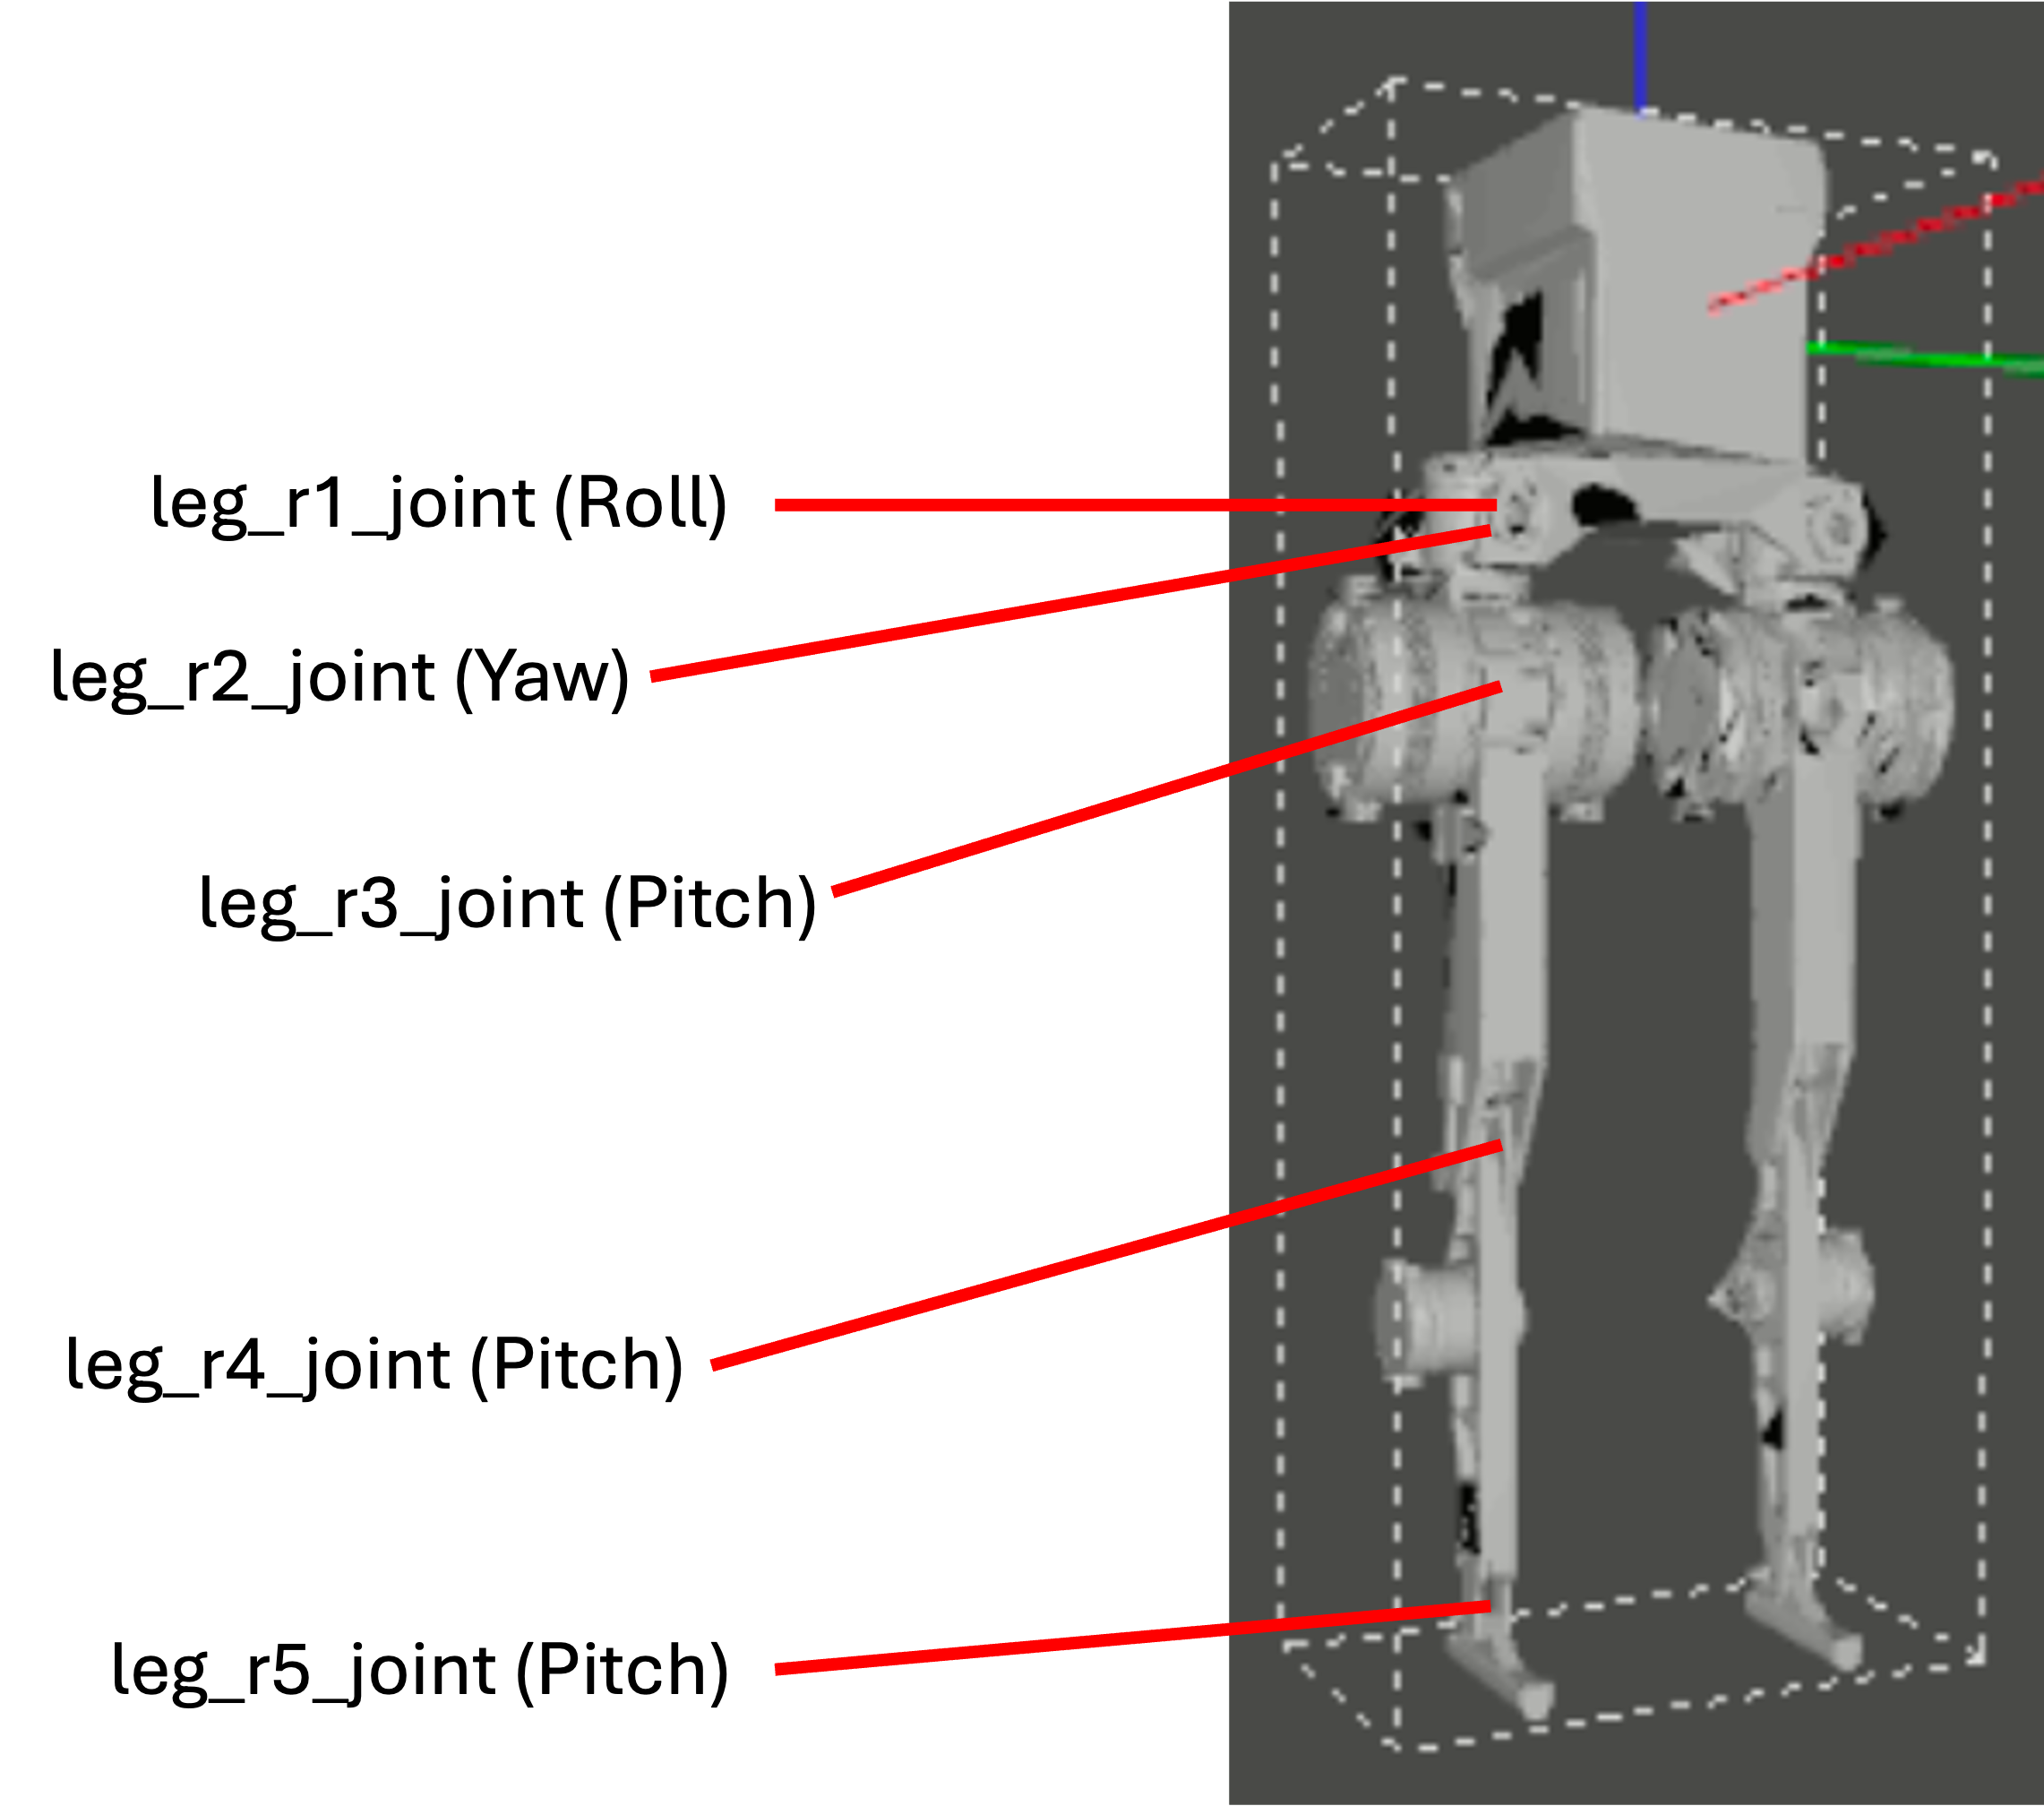
\includegraphics[width=0.85\linewidth]{hunter_robot_joints}
    \footnotesize{Hunter Robot Joint Configuration}
\end{center}

\textbf{Joint Mapping:}
\begin{itemize}\compresslist
    \item Hip: Roll, Yaw, Pitch (3 DOF/leg)
    \item Knee: Flexion (1 DOF/leg) 
    \item Ankle: Dorsiflexion (1 DOF/leg)
\end{itemize}
}

\headerbox{3. Contribution: Three-Stage Curriculum Learning}{name=curriculum,column=1,below=introduction,span=2}{

Our approach progressively increases environmental complexity to develop robust locomotion skills:

\vspace{-1.5em}
\begin{center}
\small
\begin{adjustbox}{max width=\linewidth}
\begin{tabular}{|c|c|c|c|c|c|c|}
  \hline
  \textbf{Stage} & \textbf{Environment} & \textbf{Terrain Properties} & \textbf{Domain Randomization} & \textbf{Reward Function} & \textbf{Skills Developed} & \textbf{Training Purpose} \\
  \hline
  \textbf{Stage 0} & Plane Terrain & • Mesh: plane & None & Standard locomotion & • Basic bipedal gait & Foundation stage for \\
  & (Rigid surface) & • Friction: 1.0/1.0 & • Push disturbances & rewards & • Joint coordination & loading pretrained models \\
  & & • Restitution: 0.0 & • No parameter variation & • Target height: 0.6m & • Velocity tracking & • Establishes baseline \\
  & & • High stability & • Consistent conditions & • Contact force limit: 100N & • Balance control & walking patterns \\
  \hline
  \textbf{Stage 1} & Soft Soil & • Mesh: heightfield & None & Soil-adapted rewards & • Adaptive foot placement & Introduces soil physics \\
  & (Deformable surface) & • Young's modulus: 1.0e7 & • No randomization & • Adjusted height: 0.56m & • Force modulation & without complexity of \\
  & & • Contact stiffness: 1.0e5 & • Consistent soil properties & • Contact force limit: 300N & • Compliant surface gait & randomization \\
  & & • Cohesion: 1.0e4 & • Stable learning conditions & • Reduced penalties & • Soil sinkage adaptation & • Smooth progression \\
  & & • Friction: 0.60/0.45 & & for slip/orientation & & from rigid to soft \\
  \hline
  \textbf{Stage 2} & Farm Soil & • Same soil physics & Full randomization & Same as Stage 1 & • Robust terrain adaptation & Maximum robustness \\
  & (Agricultural terrain) & • Terrain amplitude: 0.015 & • Push disturbances: disabled & • Handles variability & • Multi-modal locomotion & training with all \\
  & & • Perlin noise generation & • Terrain property variation & • Maintains tracking & • Environmental adaptation & environmental variations \\
  & & • 8x8m terrain grid & • Friction range: [0.50,0.70] & performance under & • Disturbance rejection & • Prepares for real-world \\
  & & • 64x64 resolution & • Cohesion range: [5k,15k] & uncertainty & • Parameter robustness & deployment \\
  \hline
\end{tabular}
\end{adjustbox}
\end{center}

\vspace{-2em}
\begin{center}
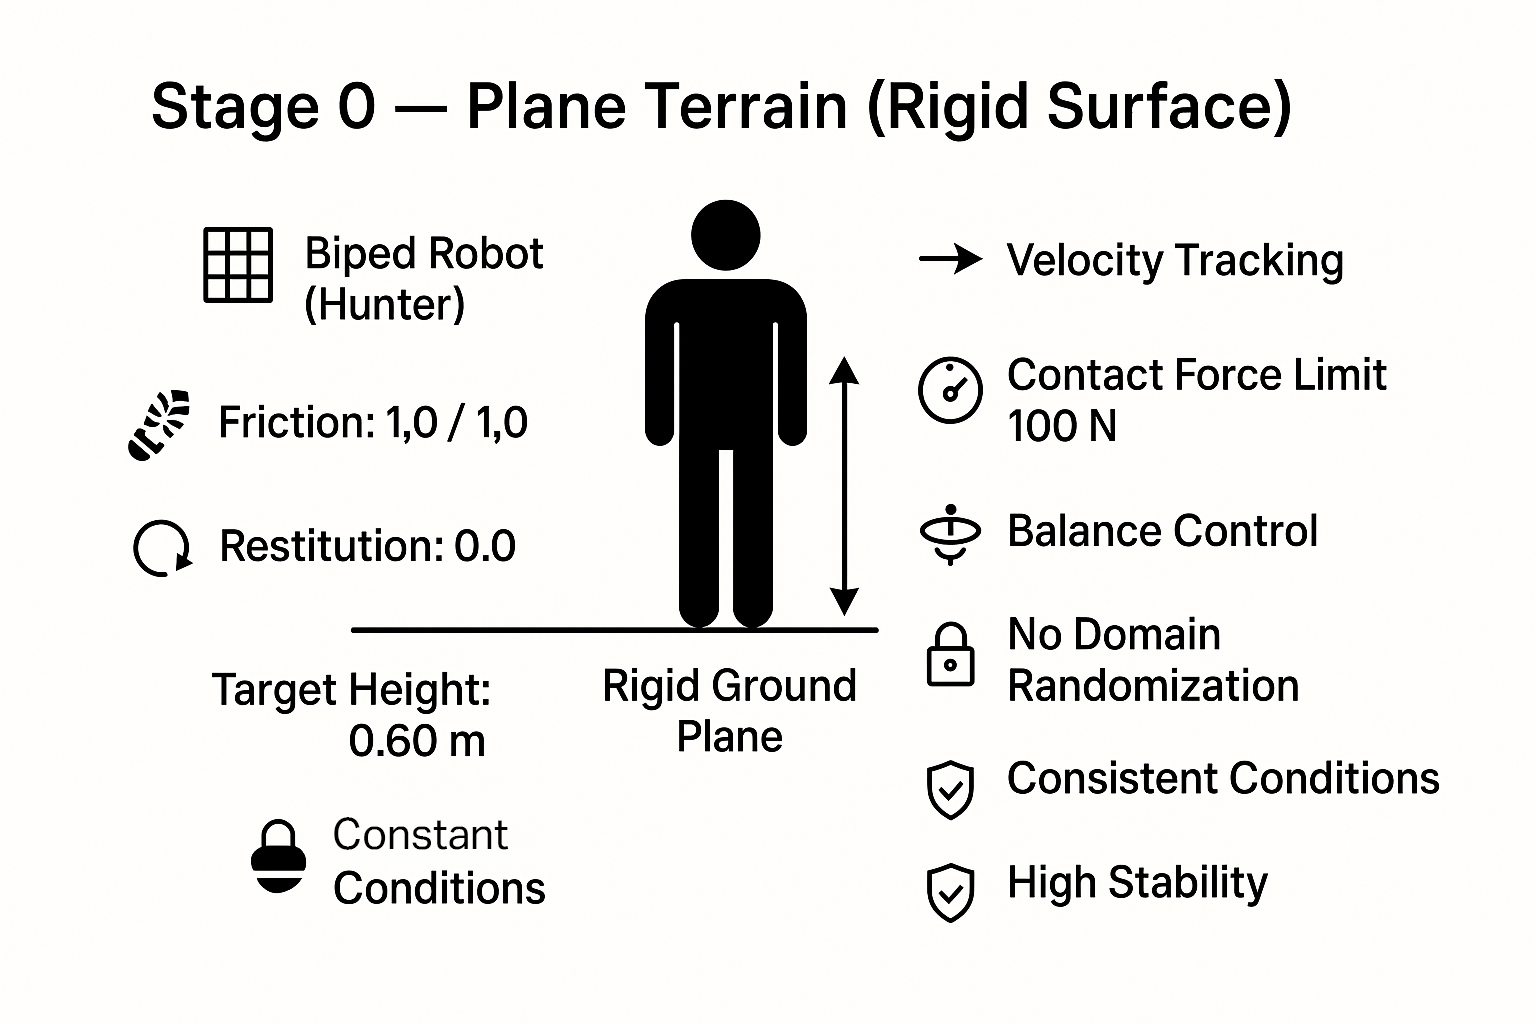
\includegraphics[width=0.3\textwidth]{stage_0.png}
\hspace{0.02\textwidth}
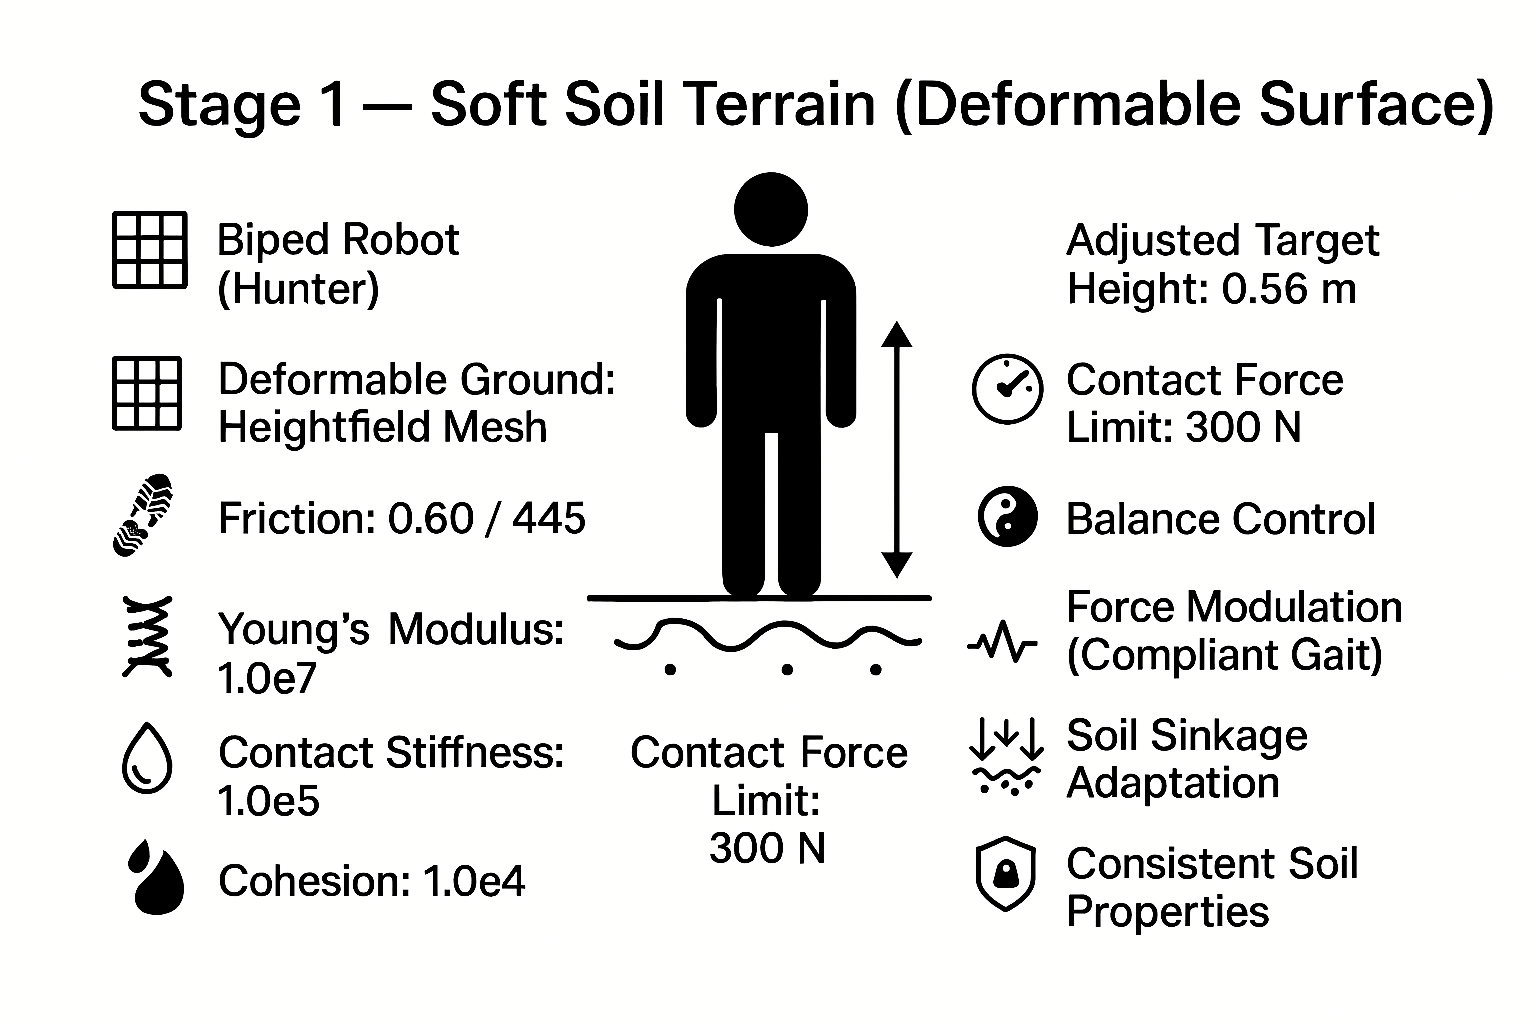
\includegraphics[width=0.3\textwidth]{stage_1.png}
\hspace{0.02\textwidth}
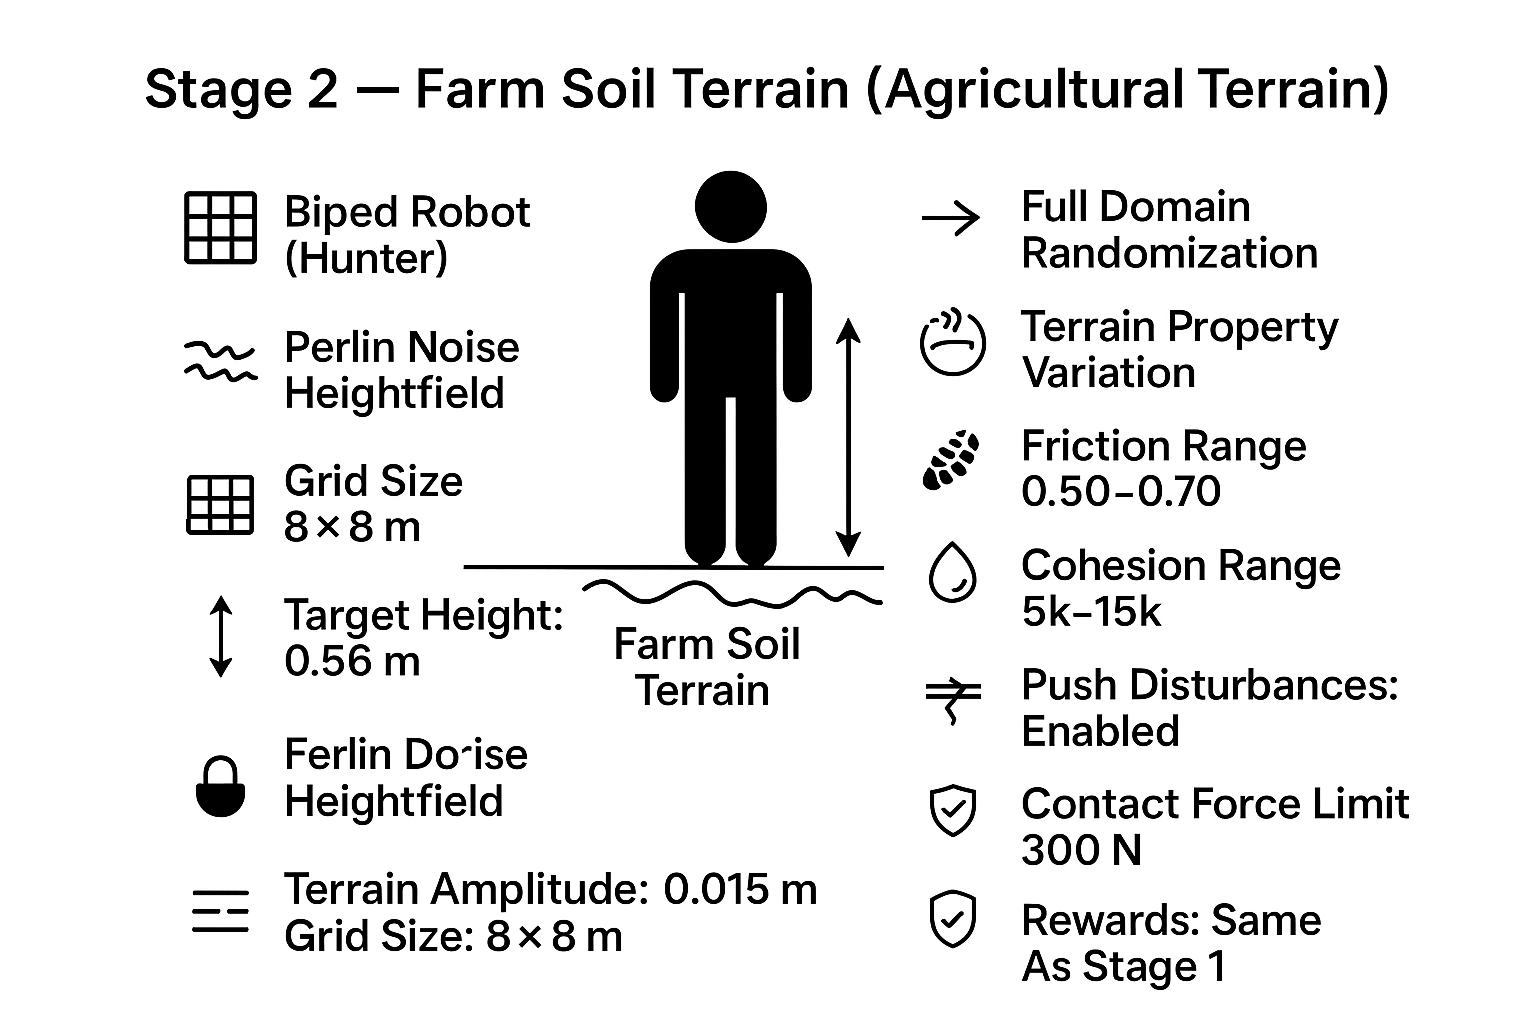
\includegraphics[width=0.3\textwidth]{stage_2.png}
\end{center}

\vspace{-3.5em}
\begin{multicols}{2}
\footnotesize
\textbf{Our contributions:}
\begin{itemize}\compresslist
    \item Introduce a three-stage soil-aware curriculum (rigid $\rightarrow$ soft soil $\rightarrow$ farm soil)
    \item Design soil-tuned rewards and PD gains
    \item Demonstrate robust biped locomotion in photorealistic Isaac Sim farm-soil with push recovery-targeting agricultural robots
\end{itemize}

\columnbreak

\textbf{Progressive Learning Benefits:}
\begin{itemize}\compresslist
    \item Stable foundation building in Stage 0
    \item Gradual complexity introduction prevents training instabilities
    \item Transfer learning between stages accelerates convergence
    \item Final policy generalizes across diverse soil conditions
\end{itemize}
\end{multicols}

}

% 4. Deep RL Architecture
\headerbox{4. Deep RL Architecture}{name=architecture,column=0,below=robot,span=1}{

\small
\textbf{Algorithm:} Proximal Policy Optimization (PPO)

\textbf{Neural Network:}
\begin{itemize}\compresslist
    \item Actor: 512→256→128 (ELU activation)
    \item Critic: 512→256→128 (ELU activation)  
    \item Output: 10D action space (joint commands)
\end{itemize}

\textbf{Key Reward Components:}
\begin{itemize}\compresslist
    \item \textbf{Tracking:} Linear/angular velocity following
    \item \textbf{Stability:} Orientation and height maintenance  
    \item \textbf{Energy:} Torque and acceleration penalties
    \item \textbf{Contact:} Proper foot placement rewards
    \item \textbf{Safety:} Joint limits and collision avoidance
\end{itemize}

\textbf{Observation Space (45D):}
\begin{itemize}\compresslist
    \item Base orientation, velocity
    \item Joint positions, velocities  
    \item Contact states
    \item Command targets
\end{itemize}
}

\headerbox{7. Experiments}{name=results,span=2,column=1,below=curriculum}{

\begin{center}
    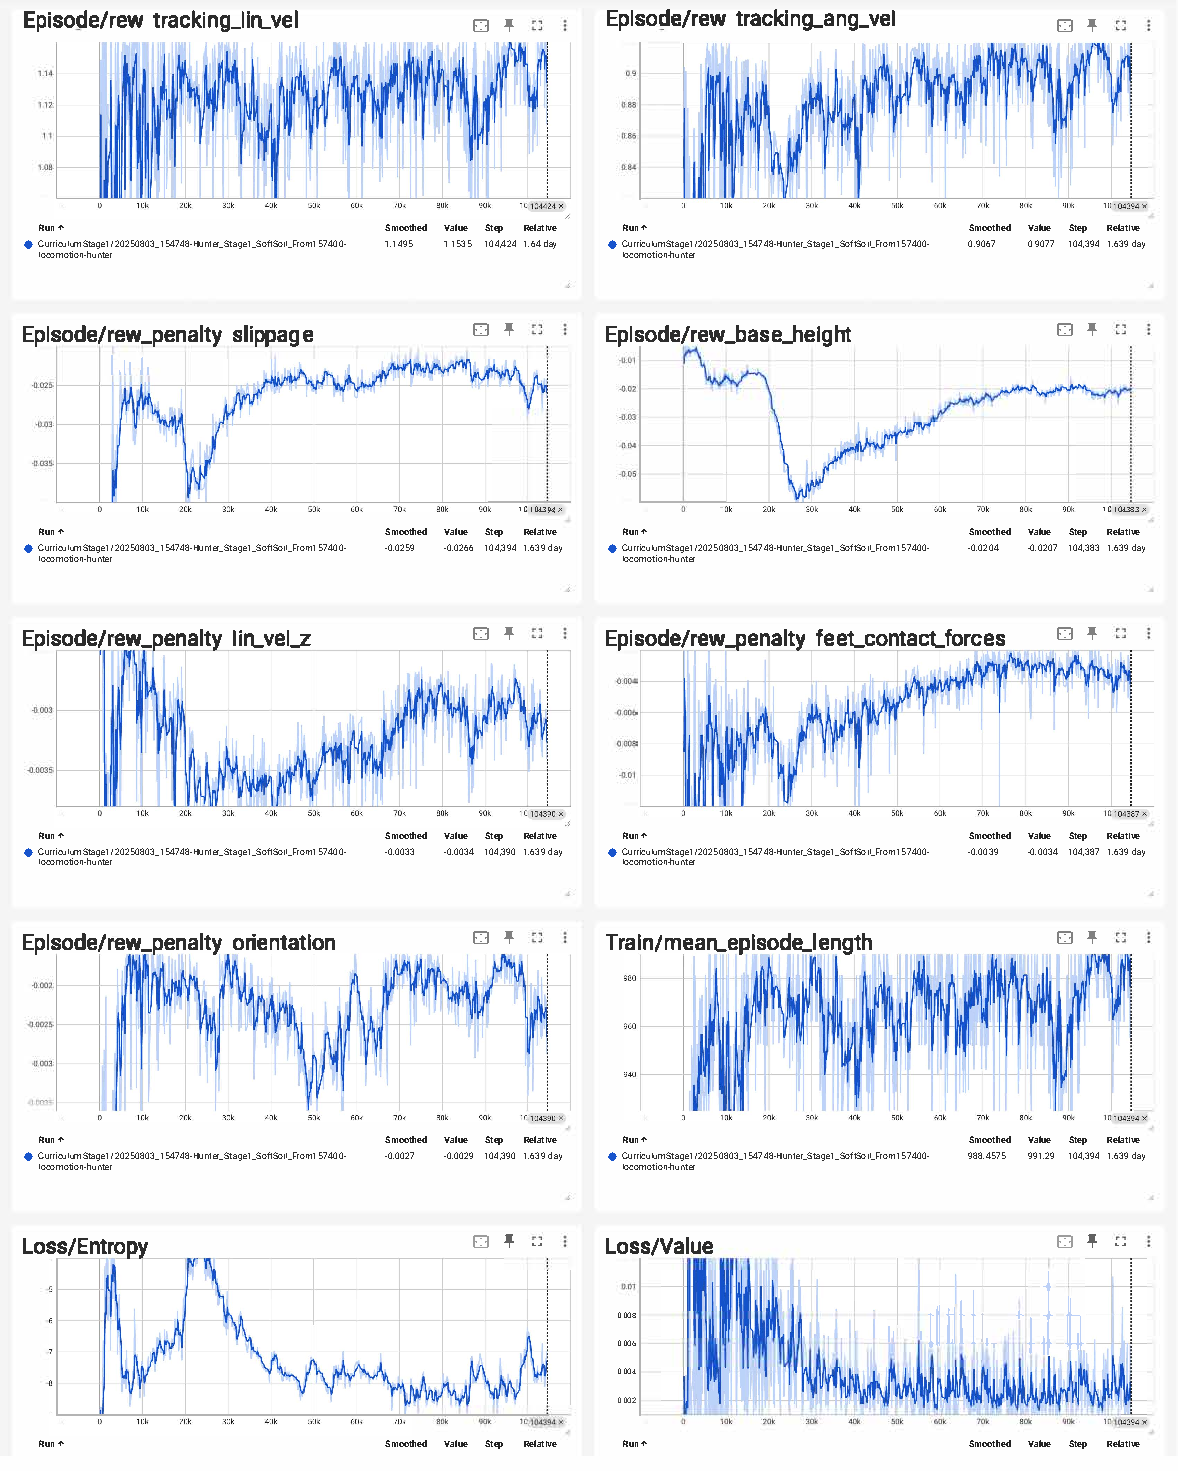
\includegraphics[width=0.47\linewidth]{learning_curves_stage1}
    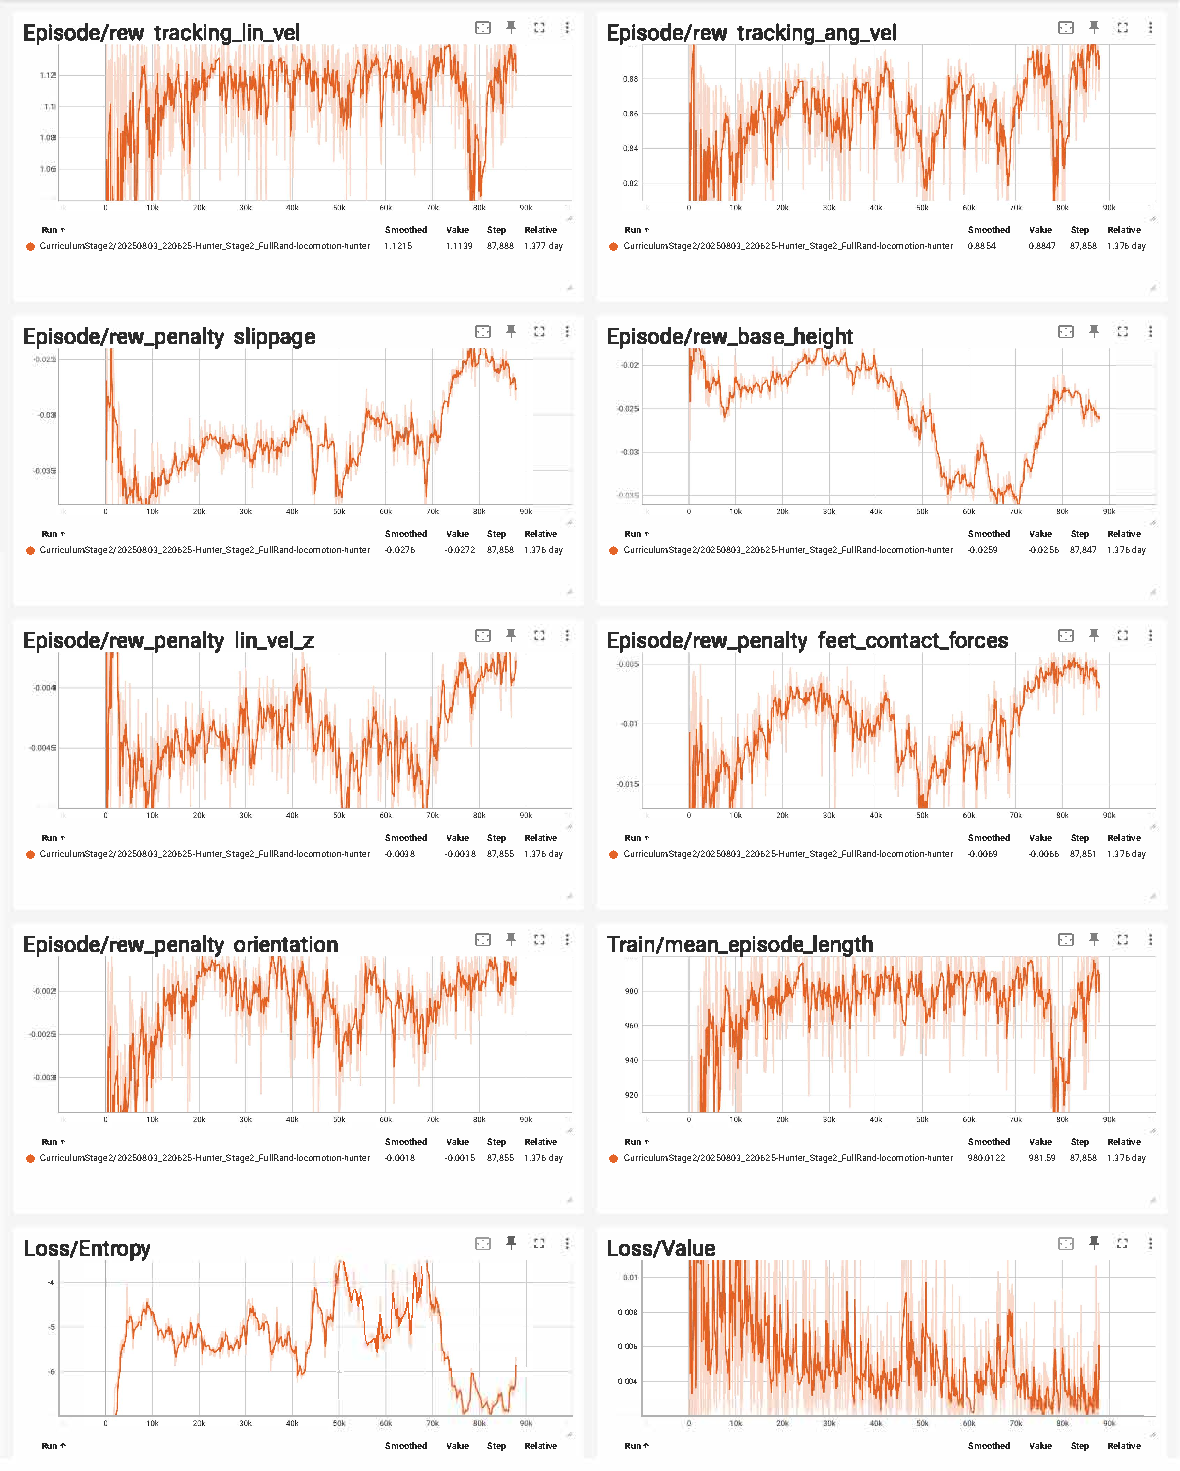
\includegraphics[width=0.47\linewidth]{learning_curves_stage2}
    
    \footnotesize{Learning curves (left is stage 1, right is stage 2) showing rewards convergence.}
\end{center}

\vspace{-1.0em}
\begin{minipage}[t]{0.47\linewidth}
\footnotesize
\textbf{Key Training Achievements:}
\begin{itemize}\compresslist
    \item Successful locomotion learning within $\approx 100K$ iterations
    \item Stable upright posture maintenance (base\_height penalty minimized)
    \item Effective velocity tracking (tracking rewards maximized)
    \item Energy-efficient gait patterns (torque penalties reduced)
    \item Robust balance control under external disturbances (0.5 m/s push resistance)
\end{itemize}
\end{minipage}
\hfill
\begin{minipage}[t]{0.47\linewidth}
\footnotesize
\textbf{Performance Metrics:}
\begin{itemize}\compresslist
    \item Walking speed: ±0.5 m/s target tracking
    \item Episode length: 20 seconds (1000 control steps at 50 Hz)
    \item Success rate: >90\% episode completion
    \item Balance recovery: Maintains stability under lateral pushes
\end{itemize}
\end{minipage}
}

\headerbox{8. Soil Adaptation Capabilities}{name=applications,span=1,column=1,below=results,above=bottom}{
\footnotesize
\begin{center}
    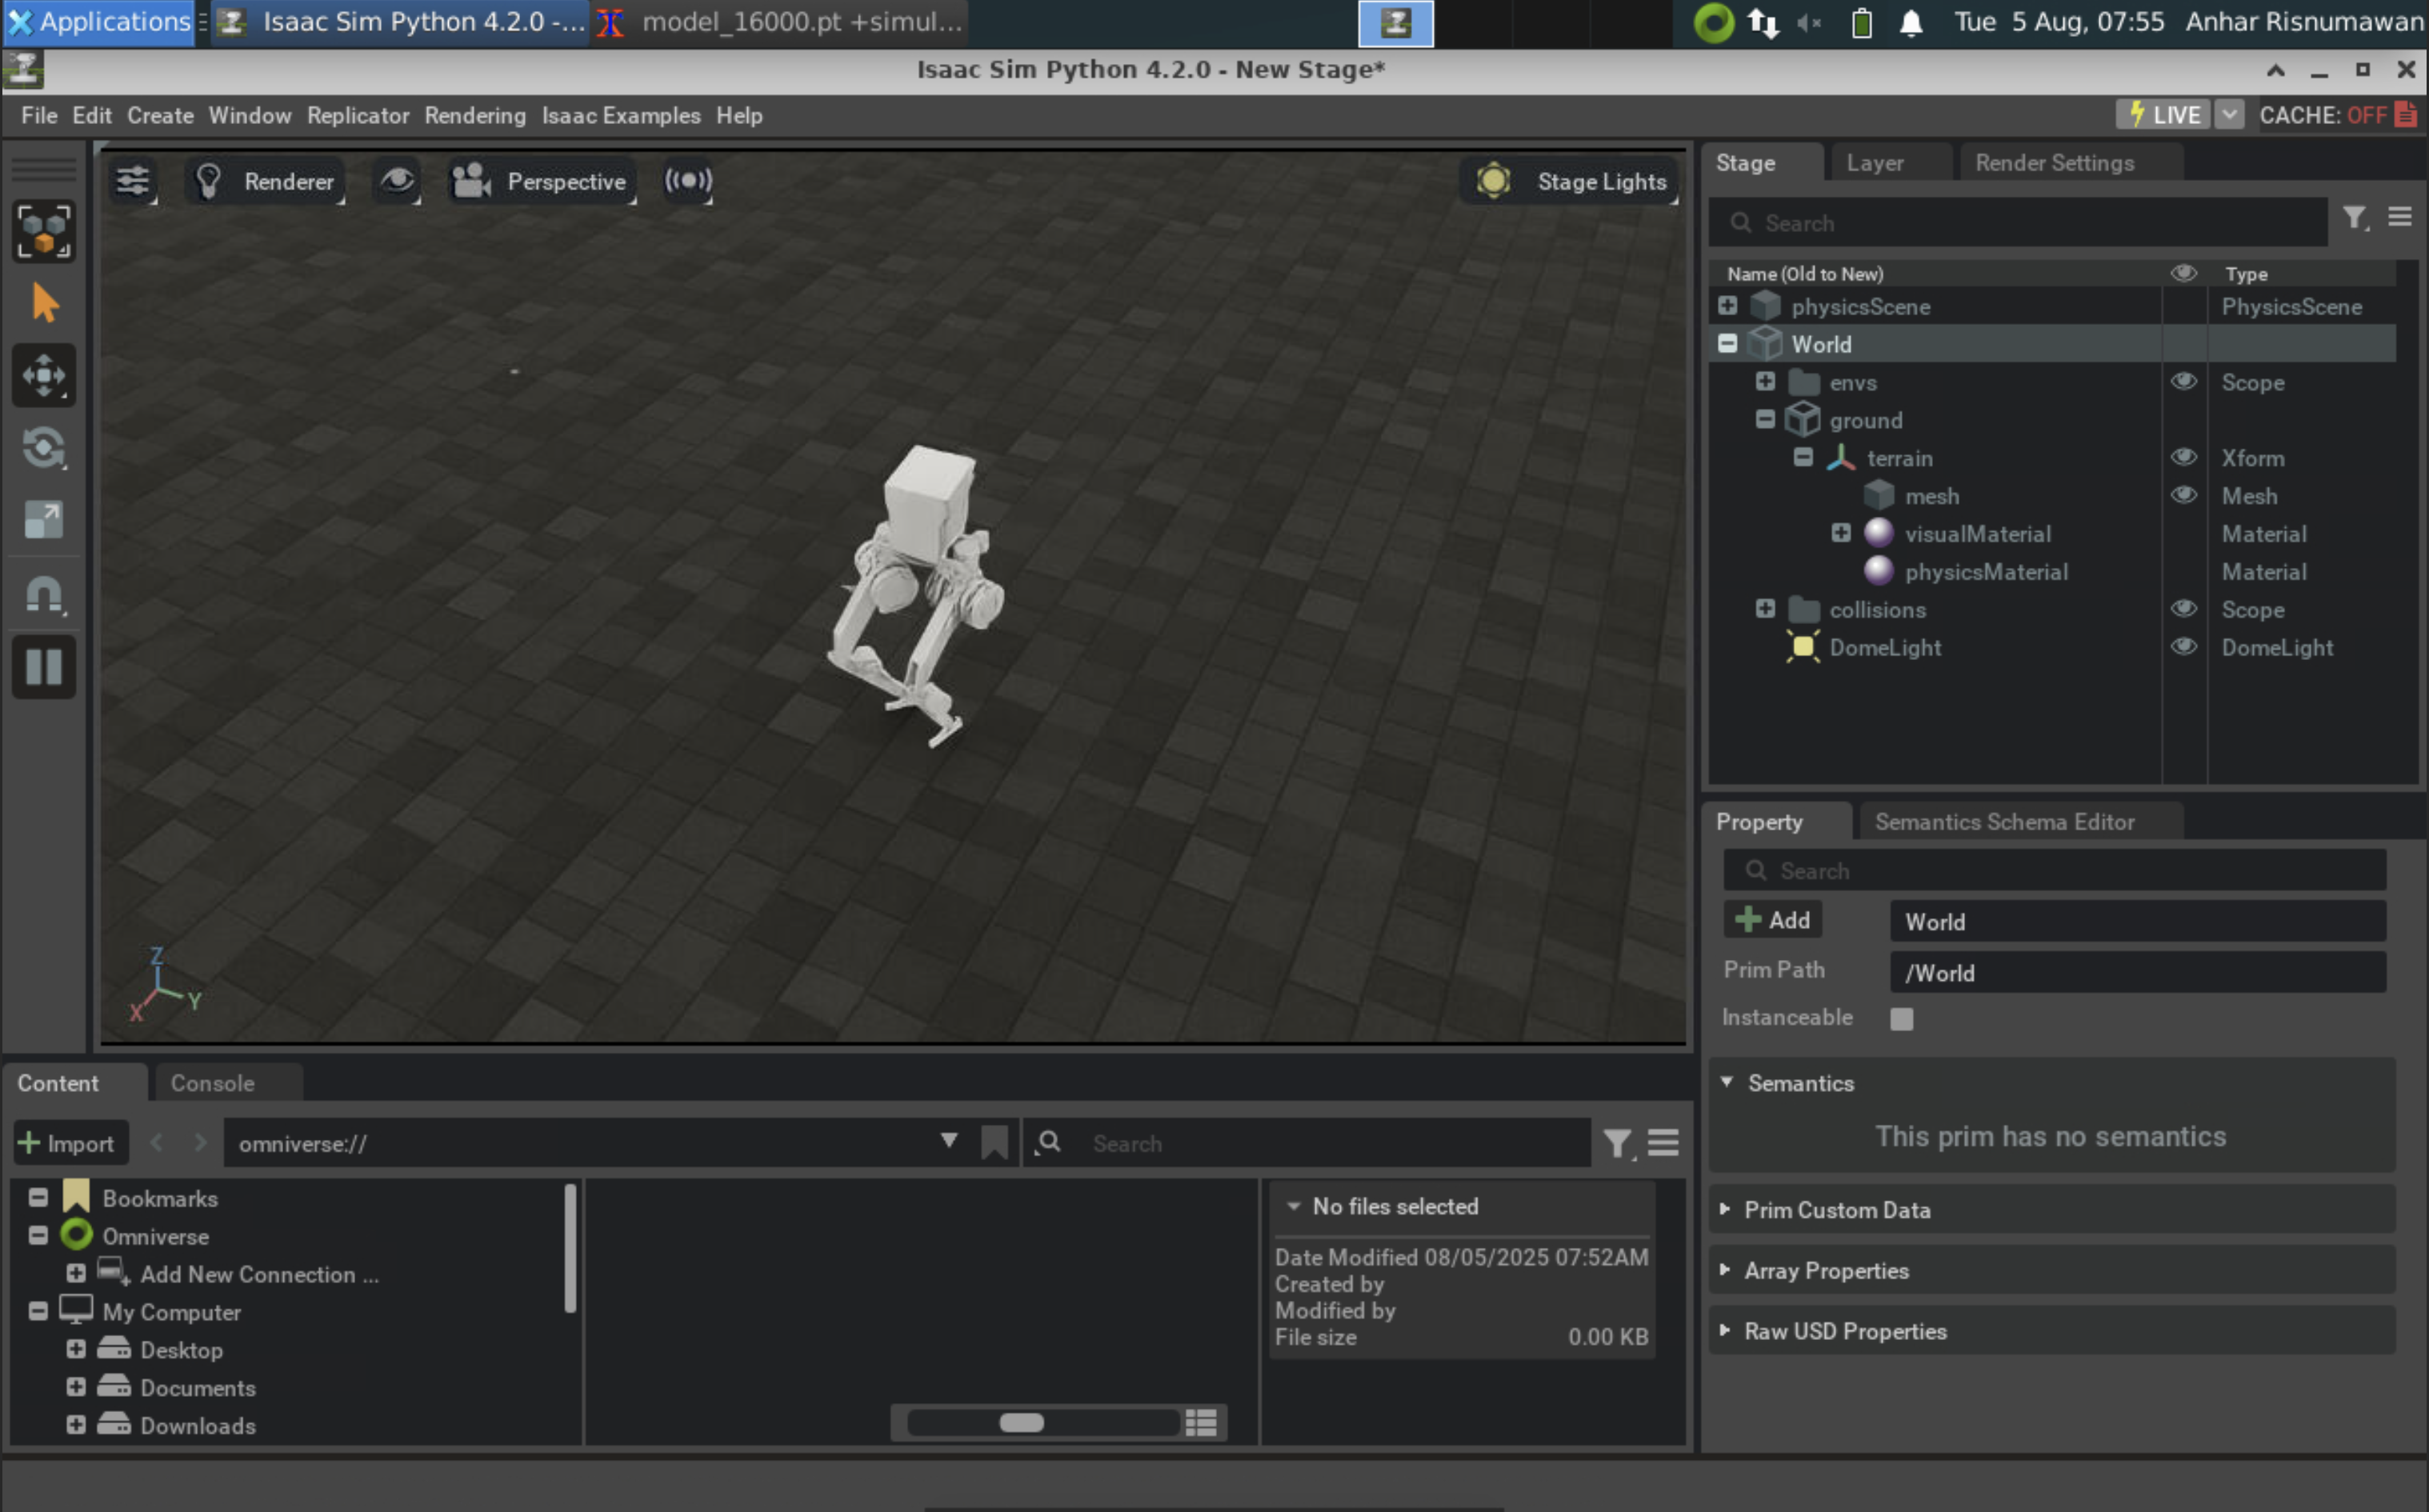
\includegraphics[width=0.95\linewidth]{hunter_soil_env}
    \footnotesize{Hunter robot navigating across different soil environments: plane terrain → soft soil → farm soil}
\end{center}

% \textbf{Stage 0 - Plane Terrain Mastery:}
% \begin{itemize}\compresslist
%     \item Achieved stable bipedal walking on rigid surfaces
%     \item Developed fundamental gait patterns and joint coordination
%     \item Established baseline locomotion behaviors for transfer learning
% \end{itemize}

% \textbf{Stage 1 - Soft Soil Adaptation:}
% \begin{itemize}\compresslist
%     \item Learning to modulate contact forces for deformable terrain
%     \item Adaptive foot placement strategies for unstable ground
%     \item Enhanced proprioceptive feedback processing for terrain sensing
% \end{itemize}

\vspace{-0.8em}
\tiny
\textbf{Stage 2 - Farm Soil Locomotion:}
\begin{itemize}\compresslist
    \item Integration of plane terrain skills with soft soil adaptations
    \item Robust performance across wet to dry agricultural soil conditions
    \item Possible applicability for farming operations and crop monitoring
\end{itemize}

% \textbf{Agricultural Applications:}
% \begin{itemize}\compresslist
%     \item Autonomous crop inspection in variable soil conditions
%     \item Precision agriculture tasks requiring stable locomotion
%     \item Reduced soil compaction compared to wheeled vehicles
%     \item Enhanced mobility in muddy or uneven farm terrain
% \end{itemize}
}

\headerbox{5. Technical Innovations}{name=innovations,column=0,below=architecture,span=1}{

\small
\textbf{Reward System Design:}
\begin{itemize}\compresslist
    \item Multi-objective optimization balancing performance and efficiency
    \item Hierarchical penalty structure prioritizing safety
    \item Contact-aware rewards for foot-ground interaction
\end{itemize}

\textbf{Morphology Adaptation:}
\begin{itemize}\compresslist
    \item URDF standardization for policy transfer
    \item Joint limit calibration matching hardware specs
    \item Contact sensor mapping for ground interaction
\end{itemize}

\textbf{Training Optimizations:}
\begin{itemize}\compresslist
    \item Episode timing: 50 Hz control frequency
    \item Batch learning: 5 epochs per iteration
    \item Curriculum scheduling: Progressive difficulty increase
\end{itemize}
}

\headerbox{6. Related Work}{name=related,column=0,below=innovations,span=1,above=bottom,textfont=\footnotesize,contentscale=1.0}{

\vspace{1.5em}
\begin{itemize}\compresslist
    \item \textbf{Sim-to-real legged locomotion.} Learning-based controllers achieve robust quadruped locomotion in natural terrain and drastically reduced training times via massive parallelism [1,2]. Rapid Motor Adaptation handles unseen dynamics through online adaptation [3].
    \item \textbf{Deformable terrain.} High-speed locomotion on soft sand using contact-aware training highlights the need to model soil compliance [4].
    \item \textbf{Imitation and skill priors.} Motion imitation (e.g., DeepMimic) seeds policies with natural gaits that transfer well [5].
    \item \textbf{Hybrid control.} Combining RL with heuristic components can improve biped stability and sim-to-real transfer [6].
    \item \textbf{Curriculum learning.} Structured curricula enable reliable biped learning over complex terrains [7].
    \item \textbf{Humanoids on compliant ground.} Recent results demonstrate robust DRL walking on HRP-5P over uneven, compliant terrain [8].
\end{itemize}
}

\headerbox{9. Conclusions \& Future Work}{name=conclusion,column=2,below=results,span=1}{

\footnotesize
\textbf{Conclusions:}
\begin{boenumerate}\compresslist
    \item Demonstrated multistages learning for agricultural soil locomotion
    \item Successful deep RL training of Hunter biped
    \item Comprehensive reward system for bipedal stability
\end{boenumerate}

\vspace{0.3em}
\textbf{Future Directions:}
\begin{itemize}\compresslist
    \item Real hardware deployment and validation
    \item Long-duration autonomous field operations
\end{itemize}
}

\headerbox{10. References}{name=references,column=2,span=1,below=conclusion,above=bottom,textfont=\tiny,contentscale=0.9}{

\begin{enumerate}\compresslist
    \item Lee, J., et al. "Learning quadrupedal locomotion over challenging terrain." Science robotics 5.47 (2020).
    \item Rudin, N., et al. "Learning to walk in minutes using massively parallel deep reinforcement learning." arXiv:2109.11978 (2022).
    \item Kumar, A., et al. "RMA: Rapid Motor Adaptation for Legged Robots." RSS (2021).
    \item Choi, S., et al. "Learning quadrupedal locomotion over deformable terrain." Science Robotics 8.74 (2023).
    \item Peng, X. B., et al. "DeepMimic: Example-guided deep reinforcement learning of physics-based character skills." ACM TOG 37.4 (2018).
    \item Wang, Z., et al. "Hybrid locomotion control of biped robots based on reinforcement learning." IEEE TSMC 53.1 (2022).
    \item Tidd, B., et al. "Guided curriculum model-based reinforcement learning for walking on uneven terrain." IROS (2020).
    \item Singh, R., et al. "Robust humanoid locomotion using deep reinforcement learning with compliant contact models." arXiv:2501.00123 (2025).
\end{enumerate}
}

\end{poster}

\end{document}